\documentclass[]{unswthesis}
\usepackage{graphicx}
%\usepackage{mwe}
%\usepackage{kantlipsum}
\usepackage{caption}

%%% Class options:

%  undergrad (default)
%  hdr

%  11pt (default)
%  12pt

%  final (default)
%  draft

%  oneside (default for hdr)
%  twoside (default for undergrad)


%% Thesis details
\thesistitle{Managing Your Social Networking Profile}
\thesissubtitle{Enabling User-Tailored Views of Your Feed}
\thesisschool{School of Computer Science and Engineering}
%\thesisschool{School of Photovoltaic and Renewable Energy Engineering}
\thesisauthor{Geoffrey Zhu and Richard Zhang}
\thesisZid{3415440 \& 3416477}
\thesistopic{3031}  % for undergrad theses only
\thesisdegree{Bachelor of Engineering in Computer Engineering}
%\thesisdegree{Doctor of Philosophy}
\thesisdate{26th May 2015}
\thesissupervisor{Dr Hye-young Paik}% for undergrad theses only				


%% My own LaTeX macros, definitions, etc
%%%% Shortcuts
\newcommand{\num}[2]{\mbox{#1\,#2}}			% num with units

%%%% Symbols
\newcommand{\yes}{\ensuremath{\surd}\xspace}		% Tick mark
\newcommand{\no}{\ensuremath{\times}\xspace}		% Cross mark
\newcommand{\by}{\ensuremath{\times}\xspace}		% XXX x XXX
\newcommand{\bAND}{\ensuremath{\wedge}\xspace}		% Bool. /\
\newcommand{\bOR}{\ensuremath{\vee}\xspace}		% Bool. \/
\newcommand{\becomes}{\ensuremath{\rightarrow}\xspace}	% -->

%%%% Custom environments

% Centered tabular with single spacing
\newenvironment{ctabular}[1]
    {\par\begin{sspacing}\begin{center}\begin{tabular}{#1}}%
    {\end{tabular}\end{center}\end{sspacing}}


%%%% Our default level for display in TOC - subsubsections
\setcounter{tocdepth}{2}



\begin{document}

%% pages in the ``frontmatter'' section have roman numeral page number
\frontmatter  
\maketitle

%\chapter*{Abstract}\label{abstract}
The universally used platform of Social Networking Services (SNS) faces many challenges as they gain huge user bases. One such SNS known as Facebook provides a feed that is a list of all items from friends, organisations and other entities. This feed contains an enormous amount of data that must be ordered in such a way that the user is satisfied. In this thesis, we will be exploring the possibilities of user modelling being used to rank these feed items as well as verifying multiple proposed algorithms in the literature. The final outcome is a more personalised algorithm for ranking items from a user’s Facebook feed.
%\chapter*{Acknowledgements}\label{ack}

We would like to thank our supervisor Dr. Helen Paik for her constant guidance and support, and our assessor Prof. Fethi Rabhi for his advice and feedback. 
%\chapter*{Abbreviations}\label{abbr}
\begin{description}
\item[BE] Bachelor of Engineering
\item[EE\&T] School of Electrical Engineering and Telecommunication
\item[\LaTeX] A document preparation computer program
\item[PhD] Doctor of Philosophy
\end{description}

\begin{itemize}
  \item Place any abbreviations we use here
\ldots
\end{itemize}


\tableofcontents
%\listoffigures  % if required

% Image Example
%\begin{figure}[ht!]
%\centering
%\graphicspath{{images/} }
%
\includegraphics{dog.jpg}
%\end{figure}

%\begin{itemize}
 % \item May not have any figures or place figures we refer to from our background reasearch
%\ldots
%\end{itemize}

%\listoftables  % if required

%\begin{itemize}
 % \item May not have any tables or place tables we refer to from our background reasearch
%\ldots
%\end{itemize}

%% pages in the ``mainmatter'' section have arabic page numbers and chapters are numbered
\mainmatter

\chapter{Introduction}\label{ch:intro}

Social Networking Services (SNS) are platforms in which a diverse range of users are able share their interests, organise social activities and keep in touch with people. In almost all SNS, users are presented with a \textit{feed}; this feed is a list of items generated via the user's connections throughout the SNS. The feed acts as a summary of activities that the user has subscribed to, a dashboard presented to them when they first log in. This feed contains a large amount of items that we would like to order, or rank in some way such that the items that the user finds more interesting have a higher precedence in the feed. As the use of SNS grows rapidly, so does the demand for such ranking algorithms.

While there exists many SNS currently being used, the scope of this thesis will be reduced to focus on only one of them; Facebook. This is mainly due to the time constraints involved, however the results and methodology used in both our research and implementation will be generalisable to all SNS. There are two main reasons why Facebook has been chosen as our SNS of focus.

Firstly, Facebook is currently the most used SNS; Statistica~\cite{statistica2015facebook} gives us the number of Facebook users for the second quarter of 2015 as almost 1.5 billion. This allows us to more easily gather users for our research purposes as well as have more confidence that our results can be generalised to most SNS.

Secondly, Facebook attracts many different types of users due to it's very flexible, generic nature (i.e. not a niche SNS). Each type of user will have different requirements and by having a large set of user types, we are able to more easily identify and distinguish them from one another.

With all this considered, it is clearly not possible to have one single ranking algorithm to accommodate for all users, and yet as of now, Facebook only offers one ranking, or view of a user's feed (besides chronological order). Our aim can be summarised as follows: First we will set out to identify these different user types and their needs, then we aim to create a number of different ranking algorithms based on the discovered user types. Thus offering a more personalised ranking of a user's feed. It is important to note that we do not aim to create a \textit{better} ranking algorithm than Facebook as an enormous amount of research and time has already been put into creating said algorithm, instead we aim to offer different, more personalised rankings.

%Chapter~\ref{ch:background} explains the background for this document.
%Chapter~\ref{ch:style} states the style and submission related requirements
%to theses submitted at the school.
%Chapter~\ref{ch:content} explains content related requirements to theses.
%Chapter~\ref{ch:eval} evaluates the thesis requirements template.  Finally,
%Chapter~\ref{ch:conclusion} draws up conclusions and suggest ways to
%further improve the thesis requirements template.


\chapter{Background}\label{ch:background}

%Every semester, students ask their supervisor how to write their thesis,
%what the requirements are, and what to write in it.  
%This document tries to answer all such questions.

\section{User Modelling}

As mentioned earlier, the first half of our approach is to identify different types of Facebook users and determine what preferences they have in terms of feed objects. We took a look to the literature to see if anyone had attempted user modelling for this purpose.
The first question we set out to answer was quite intuitive, that being what are the reasons why people use Facebook? Or even SNS in general.  Bon~\cite{bonds2010myspace} conducted  a survey on university students to confirm the results of a research paper published in 2008 which found that the main reasons people used social networks were:

\begin{itemize}
 \item Keeping in touch with friends
 \item Meeting new people
 \item Posting and looking at pictures
\end{itemize}


Factor analysis was performed on the survey answers and the results were tabulated into a list of loadings, representing how much certain features acted as the reason for the use of social networks. These results however, proved to be too general for our purposes as we are looking to define different, more concrete user types. On top of this, the scope of this Survey was restricted only to university students and contained a relatively small sample size of 200. 

%\begin{wrapfigure}[bp!]
%\graphicspath{images/}
%\centerline{
%	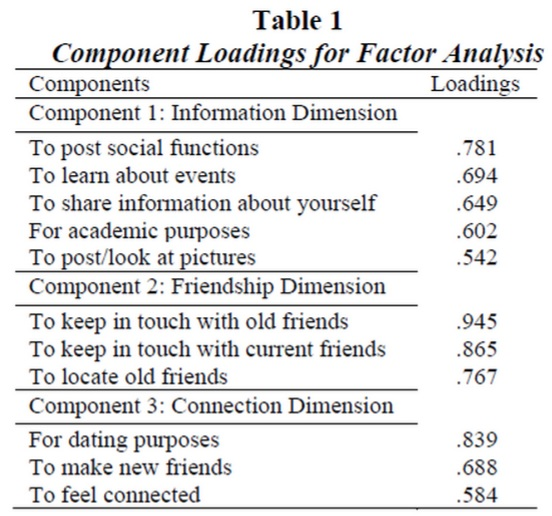
\includegraphics[width=90mm]{images/factoranalysis.jpg}
%	Figure 
%}
%\caption{Survey Results}
%\end{wrapfigure}

\begin{center}
  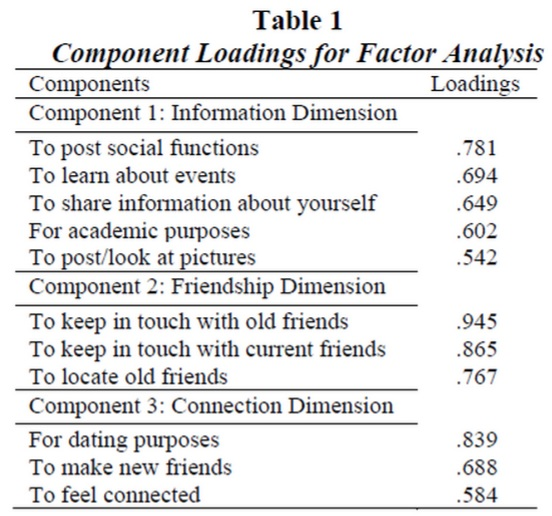
\includegraphics[scale=0.6]{images/factoranalysis.jpg}
  \captionof{figure}{Survey Results}
\end{center}

Some interesting correlations were found with further statistical analysis, for example; men significantly used social networks more for the purpose of sharing personal information and dating compared to women. While being somewhat more specific, these correlations are still slightly too generalised. However, this being said, knowing some of the more common reasons that people use Facebook will give us direction in terms of what types of feed objects we should be looking for.

Nad~\cite{nadkarni2012people} published a literature review which looked at user modelling Facebook users from a more psychological frame of view. They found that there were correlations between certain Facebook behavioural patterns and a uer's psychology. Some of the correlations that were found were:

\begin{itemize}
 \item Users with higher levels of extraversion tended to use Facebook as more of a social tool rather than to replace social activities. They also generally had accumulated more social networking friends  and had more addictive tendencies when it came to Facebook use 
 \item Users with higher levels of Neuroticism Levels tended to prefer reading information in their feed whereas users with lower levels of neuroticism preferred seeing photos
 \item Users with significantly high or low levels of neuroticism tend to be more open to share personal information on their profiles
\end{itemize}

These findings are closer to what we are looking for, however, it is not easy to determine the psychology of a user for the application of ranking their Facebook feed. However, once again, these results allow us to get a better idea of the different types of feed objects that are to be considered, for example information vs photos. 

It eventually became clear to us that even if we were to use these results for our user modelling, it is uncertain whether they are still relevant, as we saw, the survey conducted by Bon~\cite{bonds2010myspace} set out to confirm results from a study just 2 years previous to his research paper and already found that user's behaviour changed. So we began to look at how people perform user modelling and the practices involved with it. Cle~\cite{clemmensen2004four} conducted an interview with 4 different HCI proffessionals based in Sweden to gain insight into there methodologies and phylosophies. The following methods of performing user modelling that came from the interviews especially interested us and will most likely be used throughout our implementation:

\begin{itemize}
 \item Usability Tests - Observing how a user interacts with a system and asking good questions to extract meaningful feedback from the user.
 \item Surveying - Simply asking existing users questions that will aid us in our user modelling - as seen in the survey conducted by Bon~\cite{bonds2010myspace}
 \item Conceptualise how users are represented in the system (as data) - By thinking about how a user's preferences will be represented in the system itself, we are able to design our algorithms accordingly
 \item Creating personas and use cases/scenario - Designing a fictional character who would benefit from our system and creating a use case around it; this allows us to consider all the different types of users that can be modelled
\end{itemize}

With this information in mind, we have chosen to conduct another survey similar to the ones performed in the literature; to help deermine whether there are certain patterns in feed preferences for users and to group those patterns into user types. For example, if we find that there is a pattern of users that prefer to see friend's social updates, photo's and event information, we can classify those set of preferences as a user type. The survey questions will be formulated with ideas from the past surveys that have been conducted and will serve as the basis of our user modelling.

\section{Ranking Algorithms}

A ranking algorithm will give each item a score and order them with the item with the highest score at the top and the item with the lowest score at the bottom. The score of an item will depend on a set of criteria that the ranking algorithm uses. Social networking services will use these ranking algorithms in order to provide the user with items that will interest them. Since we are focusing on Facebook, the users will be provided with a feed that contains a lot of posts that they will receive. In Li~\cite{LiTiaLee2010} paper, they discovered that there are three major factors that could affect how interesting a user may find a particular item. They are:


\begin{itemize}
 \item Topical Preference
 \item Topological Locality
 \item Social Influence
\end{itemize}

Topical reference is the idea that most users are interested in a limited range of topics. Topological locality refers to the fact that users are interested in the topics that their friends like and Social influence basically says that users are interested in famous people such as singers or actors. These factors do provide some insight on what a user likes but could be further generalised to topics that a user likes. The Topological locality does raise an interesting notion, that is, users are more likely to like a post that a friend likes. We can summarize these two into a more general categorization of Topic classification and connections. Topic classification will be classifying the topics that a user may like while connections will be a measure of how 'close' the user is with their friend based on their interactivity. 

Topic classification is quite difficult we have to generalise a topic that they may like based on the posts that they receive. In a paper by Bur~\cite{Bur2013}, they analysed twitter tweets and tried to generalise a topic based on the tweets each user received. They have analysed two types of methods. They are:
\begin{itemize}
 \item BestOverlap
 \item UserInfoBigram
\end{itemize}

The BestOverlap method attempts to gather a huge amount of tweets and look at the common words in those tweets. A topic can be generated by the word is overlapped the most across all the tweets. In regards to our algorithm where we have to look at Facebook posts, the likelihood of word overlaps across a large amount of posts is quite low. This method would not be appropriate for our purposes.

The UserInfoBigram analyses the optional text that is provided in every tweet and generalises a topic from those words. In Facebook, almost no one uses the optional text so this method will also not work.

In order to do topic classificication we looked to a paper by Szo~\cite{szomszor2008semantic} who proposed a system for defining topics of interest with the aid of Wikipedia. He collated a list of tags using a user's "tagging activity" which, for our purposes could mean commonly used words in past posts. These tags are then verified using Wikipedia to check that there indeed does exist something along the lines of the tag. Wikipedia is chosen over more formal dictionaries due the the nature of social media tags not being real words, thus many of the tags will not be able to be verified by formal dictionaries such as WordNet. Wikipedia is then traversed (from the tag's wiki page) to find a super category that the tag belongs to. For example if a user generates the tag "C++", in Wikipedia, the C++ page is a subpage of the "Programming Language Families" page. 

Since a single verified tag can have many categories and the final list ends up being dominated by the broader categories, only categories that meet either of these criteria are taken:
\begin{itemize}
 \item The tag has only 1 category
 \item The category matches the tag name exactly
 \item The category is a plural of the tag
\end{itemize}

This approach nets us a list of the users general interests, which can then be used to determine how much a certain post is related to the user's interests by observing the contents of the post and determining if they belong to any of these topics, again using Wikipedia.

Aga~\cite{Aga2014} discusses activity ranking for LinkedIn which is also a Social Networking Service. They discover two more factors that have a huge impact on whether the activity is deemed interesting or not. They used the measurement of CTR or click-through-rate which is the probability of a user clicking on the link to measure the appeal of an activity. An activity that was old had a low CTR compared to an activity that was new. It seems that the freshness of an activity or the time that the activity was made had to be taken into account in the ranking algorithm.  In the graph below, we see a drop in the CTR as time progresses.

\begin{center}
  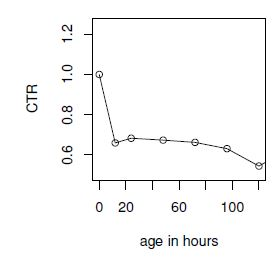
\includegraphics[scale=0.8]{images/freshness.jpg}
  \captionof{figure}{CTR vs Time Graph}
\end{center}

Another factor was diversity. A huge drop in CTR was found when they gave users a repeated type of activity in their feed. We can see this effect in the graph below. Actor repetitions refer to activites that are posted by the same user appearing in our feed.

\begin{center}
  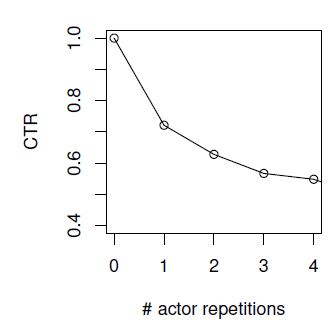
\includegraphics[scale=0.8]{images/diversity.jpg}
  \captionof{figure}{CTR vs Actor Repetitions}
\end{center}

We can surmise that freshness and diversity are key factors that must be considered in our ranking algorithm. The method that they have used to deal with these two issues involved re-ranking the feed with a decay factor to account for time and adding a negative score to activities of the same type. For our algorithm, we plan to utilise the same methods proposed as they have been successful.

Aga~\cite{Aga2014} also reinforces the idea that people are interested in what their friends like when they analysed the activities of co-workers and colleagues. Like Li~\cite{LiTiaLee2010}, they found that there was an increase in the click-through-rate of activities they were made by co-workers in the same organisation and colleagues. This emphasizes the importance of the factor of connections. We can see a huge increase in CTR in the graph below if the viewer has some relationship with the actor.

\begin{center}
  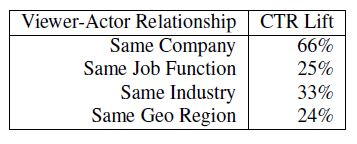
\includegraphics[scale=0.8]{images/connections.jpg}
  \captionof{figure}{Table of Relationships with CTR}
\end{center}
%\chapter{Proposal}\label{ch:proposal}

%Every semester, students ask their supervisor how to write their thesis,
%what the requirements are, and what to write in it.  
%This document tries to answer all such questions.

\section{Our Solution}

\begin{itemize}
  \item Discuss the proposal
  \item Outline differences and what we do compared to previous works
  \item explain what we want to do
\ldots
\end{itemize}

Our thesis aims to provide a more personlized view of Facebook's feed that is more adaptable to users. We do this through the introduction of user types in order to figure out what users actually want in their feed. We utilize the same tried and true algorithms used in ranking the feed but we incorporate user types and the weights that are produced from this type in order to make the feed more relevant to the user. This means that users will be provided with posts that they are more interested in at the top of their feed. 




%\usepackage{graphicx}

\chapter{Plan}\label{ch:plan}

\section{Proposal}

Our thesis aims to provide a more personlized view of Facebook's feed that is more adaptable to users. We do this through the introduction of user types in order to figure out what users actually want in their feed. We utilize the same tried and true algorithms used in ranking the feed but we incorporate user types and the weights that are produced from this type in order to make the feed more relevant to the user. This means that users will be provided with posts that they are more interested in at the top of their feed. 

\section{User Modelling}

To determine the different user types that users of our system will be able to select from, we will perform a survey spanning a variety of different topographies as mentioned in the Background Research section. If the survey results do not yield any significant preference patterns for users, we can fallback to asking users to complete a short version of our survey upon login to our system. This way, we can still generate a list of preferences for each individual user - the only tradeoff is less convenience for the user.

\section{Overall Design of the System}

\begin{center}
  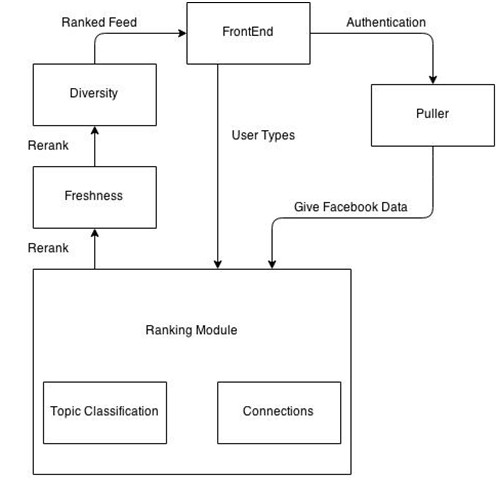
\includegraphics[scale=0.6]{images/blockdiagram.jpg}
  \captionof{figure}{Block Diagram}
\end{center}

Figure 3.1 provides a general overview of our implementation plan. It is a block diagram of our system. 

In our design, we will have a front end module which will be the website that is seen be the user. The website will have a login screen for user authentication which will allow us to pull the data from their Facebook feed. This is the job of the puller module.  The user will be given a couple of options of which user type that they think they are. The associated weights from the user types will be brought into the ranking module which contains two algorithms, one for topic classification and one for connections. The puller module will pull the feed in data into this ranking module which will rank the feed using the total scores from the topic classification, connection module and the assigned weights of the user types that came from the website or front end. To do topic classification we will look at the user's posts and try to generalise the topic based on what they have written. We will use the method proposed by Szo~\cite{szomszor2008semantic} to do topic classification.
The connections module will simply look at how often the user has interacted with the person who posted that item and give a score based on that. 

After the scores have been assigned to each post,  the feed will be ranked on the score and passed over to the freshness module. We will use Aga's~\cite{Aga2014} method and assign a decay factor to feeds that are not as recent. This feed will be reranked based on the new scores and passed over to the diversity module. In this module, we will rerank the feed and add a negative score to consecutive posts of the same type. Lastly, the newly ranked feed will be displayed in the frontend in front of the user.

We plan to use nodejs to do the whole project due to its flexibility and adaptability. We will use some written nodejs API's in order to interact with the Facebook API. 
Our timeline is shown below.

\begin{center}
  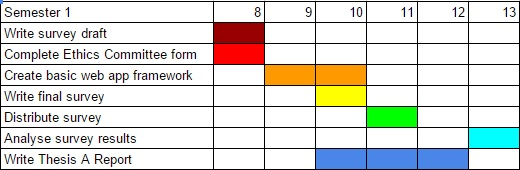
\includegraphics[scale=0.8]{images/sem1thesis.jpg}
  \captionof{figure}{Semester 1 Timeline}
\end{center}

\begin{center}
  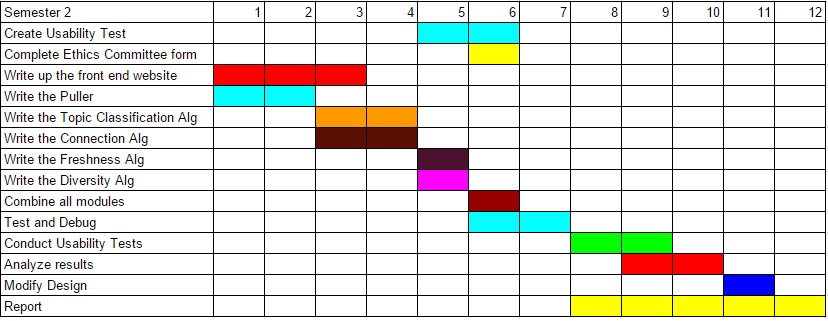
\includegraphics[scale=0.8]{images/sem2thesis.jpg}
  \captionof{figure}{Semester 2 Timeline}
\end{center}
\section {Evaluation Plan}

We considered two different ways of evaluating our system.

The first method was to simulate real users by creating Facebook accounts and attempting to mimic behaviour of each user type. We would then create a ground truth regarding how that type of user would like their feed ranked and compare the output of our ranking algorithm to the ground truth. We found quite a few flaws in this method, the major one being how difficult it would be to simulate a real user. Creating social interactions and simulating connections between users would prove very difficult. On top of this, the ground truths that we would be creating could be affected by confirmation bias. This left us with a very questionable evaluation method, so we arrived at our second one.

The second, and chosen evaluation method takes the form of gathering real users and performing a form of usability test. In this test, we will ask participants to order their feeds how they would like it to be seen, this forms an unbiased ground truth. We then run our ranking algorithm on their feeds and compare the ground truth they gave us earlier to the output. In addition to this ground truth comparison, we will ask the user to compare our ranking algorithm with the one provided by Facebook, without telling them which is which. This will give us some subjective results as to whether our ranking algorithm has succeeded in personalising the user's feed.
%\chapter{Evaluation}\label{ch:eval}

This chapter is mainly provided for the purpose of showing a typical thesis
structure.  There are no more thesis requirements described.

\section{Results}

The result of this work is the present document, being both a \LaTeX\
template and a thesis requirement specification.

\begin{itemize}
  \item The results we got
\ldots
\end{itemize}

\section{Discussion}

The Dual function of this document somewhat de-emphasises the primary
purpose of the document, namely the thesis requirements.  It would be
better, if these could be stated on a few concise pages (cf Appendix
1, p\pageref{app1}).

\begin{itemize}
  \item Discuss stuff!!
\ldots
\end{itemize}

%\chapter{Conclusion}\label{ch:conclusion}

A thesis requirements/template document has been created.  This serves the
dual purposes of giving students specific requirements to their theses ---
both style and content related --- while providing a typical thesis
structure in a \LaTeX\ template.

\begin{itemize}
  \item Do we need a conclusion for thesis A ??
  \item Summarize what we have so far??
\ldots
\end{itemize}

\section{Future Work}

Extract the requirements from the template in order to have very concise
requirements.

\begin{itemize}
  \item Possible stuff to extend our thesis
\ldots
\end{itemize}

%% chapters in the ``backmatter'' section do not have chapter numbering
%% text in the ``backmatter'' is single spaced
\backmatter
\bibliographystyle{alpha}
\bibliography{pubs}

%\chapter{Appendix 1}\label{app1}

This section contains the options for the UNSW thesis class; and
layout specifications used by this thesis.

\begin{itemize}
  \item Place all our code, pictures, everything
\ldots
\end{itemize}

\section{Options}

The standard thesis class options provided are:

\qquad
\begin{tabular}{rl}
undergrad & default \\
hdr & \\[2ex]
11pt & default\\
12pt &\\[2ex]
oneside & default for HDR theses\\
twoside & default for undergraduate theses\\[2ex]
draft & (prints DRAFT on title page and in footer and omits pictures)\\
final & default\\[2ex]
doublespacing & default\\
singlespacing & (only for use while drafting)
\end{tabular}

\section{Margins}

The standard margins for theses in Engineering are as follows:

\qquad
\begin{tabular}{|l|r|r|}
\hline
 & U'grad & HDR\\\hline
{\verb+\oddsidemargin+} & \unit[40]{mm} & \unit[40]{mm}\\
{\verb+\evensidemargin+} & \unit[25]{mm} & \unit[20]{mm}\\
{\verb+\topmargin+} & \unit[25]{mm} & \unit[30]{mm}\\
{\verb+\headheight+} & \unit[40]{mm} & \unit[40]{mm}\\
{\verb+\headsep+} & \unit[40]{mm} & \unit[40]{mm}\\
{\verb+\footskip+} & \unit[15]{mm} & \unit[15]{mm}\\
{\verb+\botmargin+} & \unit[20]{mm} & \unit[20]{mm}\\
\hline
\end{tabular}

\section{Page Headers}

\subsection{Undergraduate Theses}
For undergraduate theses, the page header for odd numbers pages in the
body of the document is:

\quad\fbox{\parbox{.95\textwidth}{Author's Name\hfill \emph{The title of the thesis}}}

and on even pages is:

\quad\fbox{\parbox{.95\textwidth}{\emph{The title of the thesis}\hfill Author's Name}}

These headers are printed on all mainmatter and backmatter pages,
including the first page of chapters or appendices.

\subsection{Higher Degree Research Theses}
For postgraduate theses, the page header for the body of the document is:

\quad\fbox{\parbox{.95\textwidth}{\emph{The title of the chapter or appendix}}}

This header is printed on all mainmatter and backmatter pages,
except for the first page of chapters or appendices.

\section{Page Footers}

For all theses, the page footer consists of a centred page number.  
In the frontmatter, the page number is in roman numerals.  
In the mainmatter and backmatter sections, the page number is in arabic numerals.
Page numbers restart from 1 at the start of the mainmatter section.  

If the \textbf{draft} document option has been selected, then a ``Draft'' message is also inserted into the footer, as in:

\quad\fbox{\parbox{.95\textwidth}{\hfill 14\hfill\hbox to 0pt{\hss\textbf{Draft:} \today}}}

or, on even numbered pages in two-sided mode:

\quad\fbox{\parbox{.95\textwidth}{\leavevmode\hbox to 0pt{\textbf{Draft:} \today\hss}\hfill 14\hfill\mbox{}}}

\section{Double Spacing}
Double spacing (actualy 1.5 spacing) is used for the mainmatter section, except for
footnotes and the text for figures and table.

Single spacing is used in the frontmatter and backmatter sections.

If it is necessary to switch between single-spacing and double-spacing, the commands \verb+\ssp+ and \verb+\dsp+ can be used; or there is a \verb+sspacing+ environment to invoke single spacing and a \verb+spacing+ environment to invoke double spacing if double spacing is used for the document (otherwise it leaves it in single spacing).  Note that switching to single spacing should only be done within the spirit of this thesis class, otherwise it may breach UNSW thesis format guidelines.

\section{Files}

This description and sample of the UNSW Thesis \LaTeX\ class consists of a number of files:

\quad\begin{tabular}{rl}
unswthesis.cls & the thesis class file itself\\[2ex]
crest.pdf & the UNSW coat of arms, used by \verb+pdflatex+ \\
crest.eps & the UNSW coat of arms, used by \verb+latex+ + \verb+dvips+ \\[2ex]
dissertation-sheet.tex & formal information required by HDR theses\\[2ex]
pubs.bib & reference details for use in the bibliography\\[2ex]
sample-thesis.tex & the main file for the thesis
\end{tabular}

The file sample-thesis.tex is the main file for the current document (in use,
its name should be changed to something more meaningful).  It presents
the structure of the thesis, then includes a number of separate files
for the various content sections.  While including separate files is
not essential (it could all be in one file), using multiple files is
useful for organising complex work.

This sample thesis is typical of many theses; however, new authors should
consult with their supervisors and exercise judgement.

The included files used by this sample thesis are:

\quad\begin{tabular}[t]{r}
definitions.tex \\
abstract.tex \\
acknowledgements.tex \\
abbreviations.tex \\
introduction.tex \\
background.tex
\end{tabular}
\quad\begin{tabular}[t]{r}
mywork.tex \\
evaluation.tex \\
conclusion.tex \\
appendix1.tex \\
appendix2.tex 
\end{tabular}

These are typical; however the concepts and names
(and obviously content) of the files making up the matter of the
thesis will differ between theses.

%\chapter{Appendix 2}\label{app2}

This section contains scads of supplimentary data.

\section{Data}

Heaps and heaps and heaps and heaps and heaps and heaps of data.
Heaps and heaps and heaps and heaps and heaps and heaps of data.
Heaps and heaps and heaps and heaps and heaps and heaps of data.
Heaps and heaps and heaps and heaps and heaps and heaps of data.
Heaps and heaps and heaps and heaps and heaps and heaps of data.

Heaps and heaps and heaps and heaps and heaps and heaps of data.
Heaps and heaps and heaps and heaps and heaps and heaps of data.
Heaps and heaps and heaps and heaps and heaps and heaps of data.
Heaps and heaps and heaps and heaps and heaps and heaps of data.
Heaps and heaps and heaps and heaps and heaps and heaps of data.

Heaps and heaps and heaps and heaps and heaps and heaps of data.
Heaps and heaps and heaps and heaps and heaps and heaps of data.
Heaps and heaps and heaps and heaps and heaps and heaps of data.
Heaps and heaps and heaps and heaps and heaps and heaps of data.
Heaps and heaps and heaps and heaps and heaps and heaps of data.

Heaps and heaps and heaps and heaps and heaps and heaps of data.
Heaps and heaps and heaps and heaps and heaps and heaps of data.
Heaps and heaps and heaps and heaps and heaps and heaps of data.
Heaps and heaps and heaps and heaps and heaps and heaps of data.
Heaps and heaps and heaps and heaps and heaps and heaps of data.

Heaps and heaps and heaps and heaps and heaps and heaps of data.
Heaps and heaps and heaps and heaps and heaps and heaps of data.
Heaps and heaps and heaps and heaps and heaps and heaps of data.
Heaps and heaps and heaps and heaps and heaps and heaps of data.
Heaps and heaps and heaps and heaps and heaps and heaps of data.

Heaps and heaps and heaps and heaps and heaps and heaps of data.
Heaps and heaps and heaps and heaps and heaps and heaps of data.
Heaps and heaps and heaps and heaps and heaps and heaps of data.
Heaps and heaps and heaps and heaps and heaps and heaps of data.
Heaps and heaps and heaps and heaps and heaps and heaps of data.

Heaps and heaps and heaps and heaps and heaps and heaps of data.
Heaps and heaps and heaps and heaps and heaps and heaps of data.
Heaps and heaps and heaps and heaps and heaps and heaps of data.
Heaps and heaps and heaps and heaps and heaps and heaps of data.
Heaps and heaps and heaps and heaps and heaps and heaps of data.

Heaps and heaps and heaps and heaps and heaps and heaps of data.
Heaps and heaps and heaps and heaps and heaps and heaps of data.
Heaps and heaps and heaps and heaps and heaps and heaps of data.
Heaps and heaps and heaps and heaps and heaps and heaps of data.
Heaps and heaps and heaps and heaps and heaps and heaps of data.

Heaps and heaps and heaps and heaps and heaps and heaps of data.
Heaps and heaps and heaps and heaps and heaps and heaps of data.
Heaps and heaps and heaps and heaps and heaps and heaps of data.
Heaps and heaps and heaps and heaps and heaps and heaps of data.
Heaps and heaps and heaps and heaps and heaps and heaps of data.

Heaps and heaps and heaps and heaps and heaps and heaps of data.
Heaps and heaps and heaps and heaps and heaps and heaps of data.
Heaps and heaps and heaps and heaps and heaps and heaps of data.
Heaps and heaps and heaps and heaps and heaps and heaps of data.
Heaps and heaps and heaps and heaps and heaps and heaps of data.

Heaps and heaps and heaps and heaps and heaps and heaps of data.
Heaps and heaps and heaps and heaps and heaps and heaps of data.
Heaps and heaps and heaps and heaps and heaps and heaps of data.
Heaps and heaps and heaps and heaps and heaps and heaps of data.
Heaps and heaps and heaps and heaps and heaps and heaps of data.



\end{document}
